\chapter{Stato dell'arte}
\begin{comment}
Cosa devo mettere in questa sezione??

- L'obbiettivo è arrivare a parlare del modello LAMA e stylegan2, quindi effetturò una serie di passaggi per passare dai primi modelli gan generativi
(goodfellow2014generative) a quelli più recenti come stylegan2 (karras2019analyzing), che erano i più utilizzati per generare immagini di alta qualità fino a poco tempo fa.
Per poi passare per pix2pix per introdurre le reti generative condizionate, e quindi dopo una breve introduzione al problema dell'inpainting arrivare a parlare di LAMA.

SCALETTA:
    - first gan (goodfellow2014generative)
    - DCGAN
    - WGAN
    - StyleGAN
    - StyleGAN2
    - pix2pix
    - LAMA
\end{comment}

In questa sezione verranno mostrati i principali modelli generativi basati su architettura GAN, che sono stati utilizzati negli ultimi anni, partendo dal 
primo modello proposto da Goodfellow et al. \cite{goodfellow2014generative} capostipite di questa famiglia di modelli passando per le principali innovazioni
proposte da altri autori, fino ad arrivare a modelli più recenti come StyleGAN2 \cite{karras2020analyzing} e LAMA \cite{suvorov2021resolutionrobust}.

\section{Il primo modello gan}
Nel 2014 Ian Goodfellow et al. \cite{goodfellow2014generative} hanno proposto il primo modello generativo basato su architettura GAN (Generative Adversarial Neural Network).
Questa pubblicazione ha segnato un punto di svolta nella ricerca dei modelli di deep learning generativi, i quali fino ad allora erano
basati su architetture come gli \textit{autoencoder} o le \textit{deep Boltzmann machines} (DBM) che non sono in grado di generare dati di alta qualità,
o se arrivano a buoni risultati tipicamente hanno una distribuzione molto concentrata intorno ai dati del training set, dunque raggiungendo una scarsa generalizzazione.

\begin{comment}
    Next paragraphs:
    - che cos'è un modello generativo basato su architettura gan
        - struttura basilare (discriminator, generator).
    - come funziona il training e la loss function originaria (bce) con riferimenti al gradiente e alla necessità di un addestramento alternato
\end{comment}

\subsection{L'adversarial training}
Il modello GAN proposto in questa ricerca si componeva di due attori principali, il \textit{discriminatore} $\mathbf{D}$ e il \textit{generatore} $\mathbf{G}$
, due modelli neurali MLP, che si affrontano in un gioco a due giocatori a somma zero.
Il generatore in questo gioco ha il compito di generare dati che siano in grado di ingannare il discriminatore, che ha il compito opposto di distinguere i dati che 
provengono dal generatore da quelli che provengono dal training set. Il gioco viene detto a somma zero in quanto il successo di uno dei due attori è sempre
associato al fallimento dell'altro, dunque il gioco non può mai vedere entrambi i giocatori vincitori. 
I due diventeranno gradualmente sempre più bravi nel loro compito fino al punto
in cui la distribuzione dei dati generati dal generatore sarà molto simile a quella dei dati del training set.
Una componente importante che differenzia le GAN da altri modelli generativi è la presenza di un input random $\mathbf{z}$, che viene passato al generatore
, questo fatto porta il generatore ad una maggiore generalizzazione in quanto questo cercherà naturalmente una 
funzione che leghi il suo output ad un input random, dunque la sua distribuzione sarà più ampia e non strettamente concentrata intorno ai dati del training set
come nel case dei variational autoencoder (VAE).

A questo punto, iniziamo ad elencare le componenti che utilizzeremo per descrivere matematicamente come funziona la procedura di addestramento 
di questa GAN.

\begin{itemize}
    \item $\mathbf{x}$: data from the training set, $\mathbf{x \in \mathbb{R}^n}$.
    \item $\mathbf{z}$: input casuale, utilizzato per determinare una mappatura nello spazio dei dati, $\mathbf{z \in \mathbb{R}^m}$.
    \item $\mathbf{y}$: uscita del discriminatore, $\mathbf{y \in [0,1]}$, esprime la probabilità che x sia reale.
    \item $\mathbf{\hat{y}}$: uscita desiderata, $\mathbf{\hat{y} \in \{0,1\}}$, può assumere solo due valori, vero o falso.
    \item $\mathbf{p_z}$: distribuzione dei vettori casuali passati al generatore.
    \item $\mathbf{p_g}$: distribuzione dei dati generati dal generatore.
    \item $\mathbf{p_{_{data}}}$: distribuzione dei dati del training set.
    \item $\mathbf{\theta}_G$: parametri del generatore.
    \item $\mathbf{\theta}_D$: parametri del discriminatore.
    \item $\mathbf{G(\theta_G, z)}$: Funzione generatore che mappa lo spazio random $z$ nello spazio dei dati, attraverso i parametri $\mathbf{\theta}_G$.
    definibile come una funzione $\mathbf{f: \mathbb{R}^m \rightarrow \mathbb{R}^n}$.
    \item $\mathbf{D(\theta_D, x)}$: Funzione discriminatore che mappa lo spazio dei dati in un uno spazio $\mathbf{\{0,1\}}$, attraverso i parametri $\mathbf{\theta}_D$. 
    definibile come una funzione $\mathbf{f:} \mathbf{\mathbb{R}^n \rightarrow \{0,1\}}$. Tale spazio identifica la provenienza di un sample x come segue:
    \begin{itemize}
        \item se $\mathbf{D(\theta_D, x)} = 1 \rightarrow x \in \mathbf{p_{_{data}}}$.
        \item se $\mathbf{D(\theta_D, x)} = 0 \rightarrow x \in \mathbf{G(\theta_G, z)}$.
    \end{itemize}
\end{itemize}

    \begin{figure}[H]
        \centering
        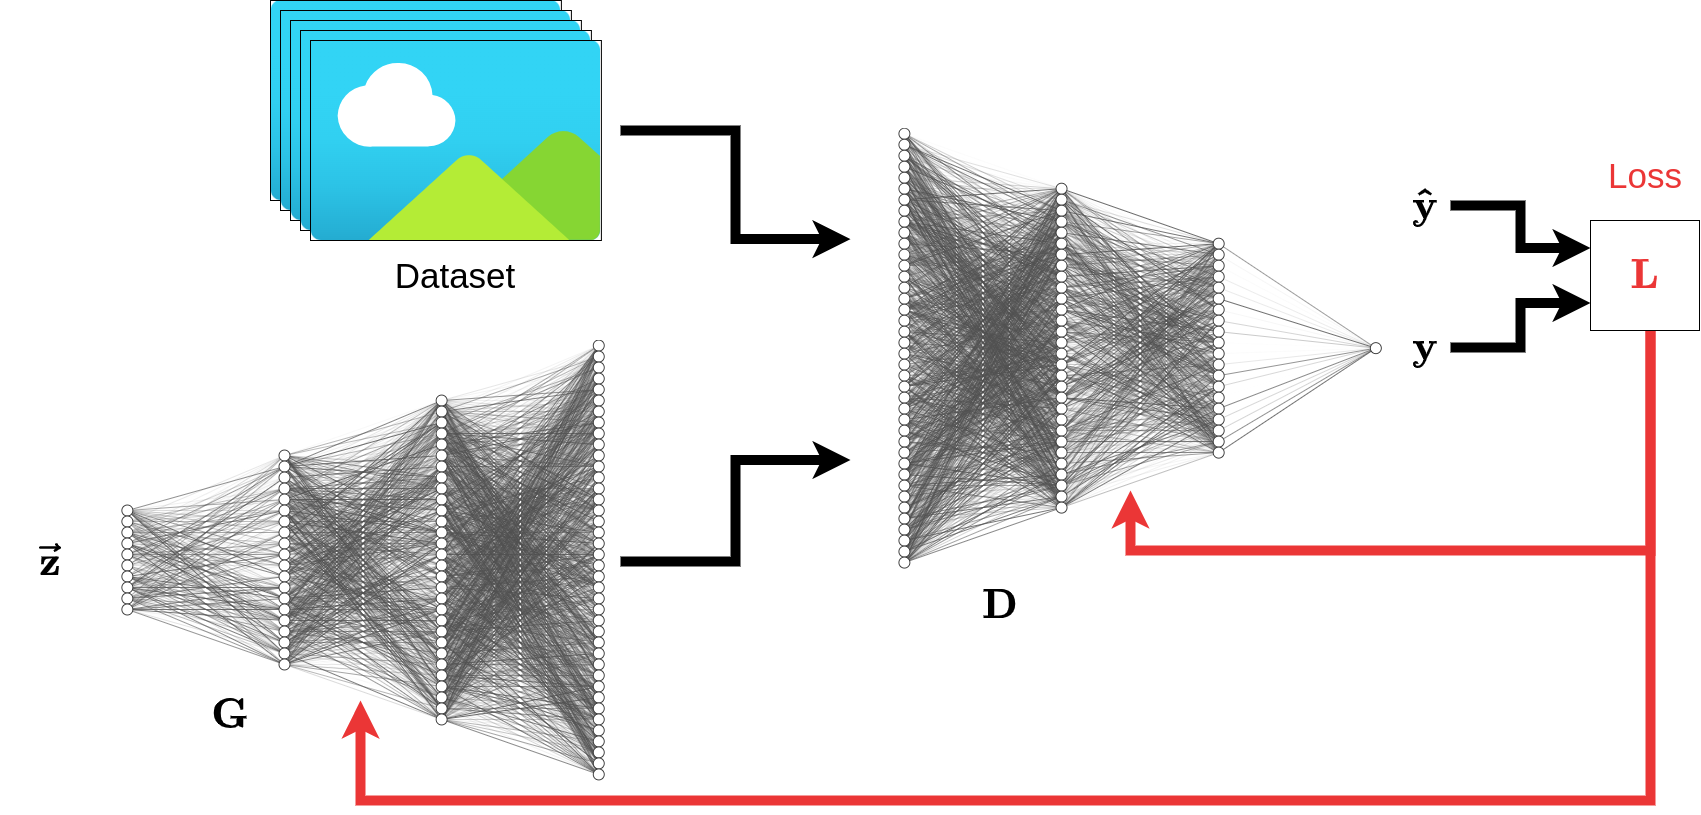
\includegraphics[width=1.0\textwidth]{imgs/GAN_training.png}
        \caption{Rappresentazione grafica della training pipeline di un modello GAN.}
        \label{fig:gan_training}
    \end{figure}

\subsection{La loss function}
Questo framework utilizza come loss function la Binary Cross Entropy (BCE), utilizzata tipicamente per la classificazione \textbf{binaria}. 
La BCE in generale è definita come segue:

\begin{equation}
    \mathbf{BCE(y, \hat{y}) = -\hat{y} \cdot \log(y) - (1-\hat{y}) \cdot \log(1-y)}
\end{equation}

Presenta 2 componenti principali, $\mathbf{-\hat{y} \cdot \log(y)}$ che si attiva quando il risultato atteso è $\mathbf{y = 1}$, mentre l'altra componente si azzera,
e $\mathbf{(1-\hat{y}) \cdot \log(1-y)}$ che si attiva quando il risultato atteso è $\mathbf{y = 0}$, con l'altra componente a 0.

\begin{figure}[H]
    \begin{tabular}{cc}
        % first row
        \vspace{0.15cm}
        \subfloat[Binary Cross Entropy ($\hat{y} = 0$)]{
            \label{fig:BCE_0}
            \centering
            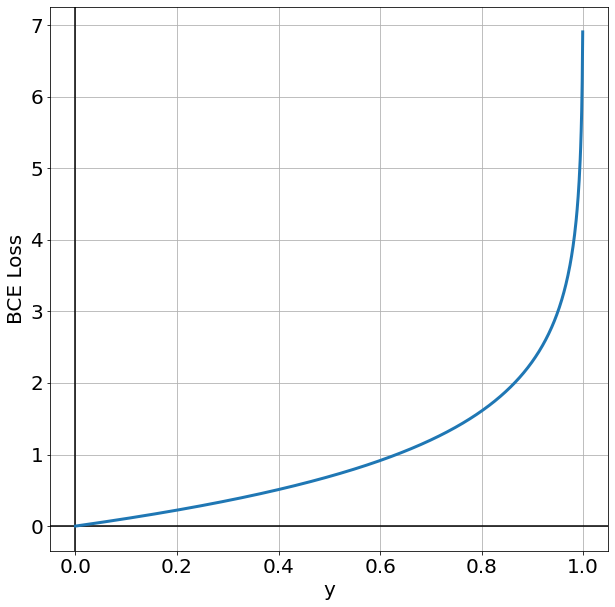
\includegraphics[width=0.4\textwidth]{imgs/graphs/bce_0.png}
        }  &
        \subfloat[Binary Cross Entropy ($\hat{y} = 1$)]{
            \label{fig:BCE_1}
            \centering
            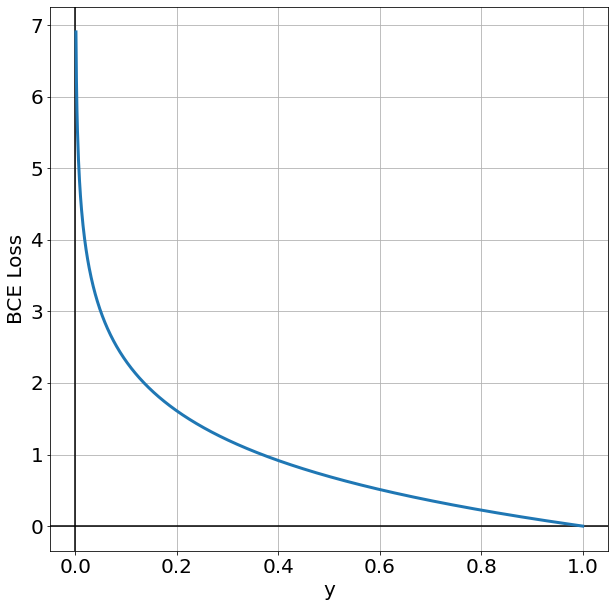
\includegraphics[width=0.4\textwidth]{imgs/graphs/bce_1.png}
        }  \\
        \vspace{0.25cm}
        \subfloat{
            \begin{tabular}{|c|}
                \hline
                $\mathbf{-\log(1-y)}$ \\
                \hline
            \end{tabular}
        } &
        \subfloat{
            \begin{tabular}{|c|}
                \hline
                $\mathbf{-\log(y)}$\\
                \hline
            \end{tabular}
        } \\
    \end{tabular}
\end{figure}

Nel caso dell'addestramento di un modello GAN, possiamo riscrivere la BCE, attuando alcune semplificazioni, e sostituendo $\mathbf{y}$
con il valore corrispondente, nel caso in cui la $\mathbf{y}$ deriva da un sample reale e quando deriva da un sample generato:

\begin{equation}
    \mathbf{\hat{y} = 1 \rightarrow y = D(\theta_D, x)}
\end{equation}

\begin{equation}
    \mathbf{\hat{y} = 0 \rightarrow y = D(\theta_D, G(\theta_G, z))}
\end{equation}

Trasformando la BCE loss in un gioco di minimizzazione e massimizzazione contrapposta tra i due attori, ottenendo la seguente funzione: 

\begin{equation}
    \mathbf{min_G max_D V(D,G) = \mathbb{E}_{x\sim p_{data}}[log(D(x))] + \mathbb{E}_{z\sim p_{z}}[log(1 - D(G(z)))]}
\end{equation}

In generale possiamo riscrivere le due componenti della funzione appena descritta in maniera estesa come segue:

\begin{equation}
    \mathbb{E}_{x\sim p_{data}}[log(D(x))] = \sum_{i=1}^{n} log(D(x_i)), x_i \in \mathbb{D}t
\end{equation}

Dove $\mathbb{D}t = \{x_1, x_2, ..., x_n\}$ è l'insieme degli esempi del training set. Mentre la seconda componente è definita come segue:

\begin{equation}
    \mathbb{E}_{z\sim p_{z}}[log(1 - D(G(z)))] = \sum_{i=1}^{n} log(1 - D(G(z_i))), z_i \sim p_{z}
\end{equation}

L'applicazione di questa funzione però necessita di qualche accorgimento, nella pratica infatti il modello viene addestrato in due fasi distinte e periodiche,
in una viene addestrato il discriminatore, e nell'altra il generatore, per un numero di step predefiniti. 
Tale dinamica di addestramento ha lo scopo di mantenere le uscite
del discriminatore per i dati generati e reali sufficientemente vicine da non causare problemi di saturazione.
Altrimenti la saturazione comporta un azzeramento del gradiente e di conseguenza un arresto dell'apprendimento.

\subsection{La convergenza del generatore}
Per visualizzare meglio le dinamiche dell'addestramento che portano alla convergenza del generatore alla distribuzione del training set 
possiamo utilizzare un grafico, ipotizzando di visualizzare i dati del training set su una sola dimensione,
e di visualizzare sull'asse y la densità di probabilità dei dati e il valore dell'uscita del discriminatore, al variare di $\mathbf{x}$, ossia
della variabile di input del discriminatore, in questo caso unidimensionale ma in generale potrebbe rappresentare immagini, audio video e così via.

\begin{figure}[H]
    \centering
    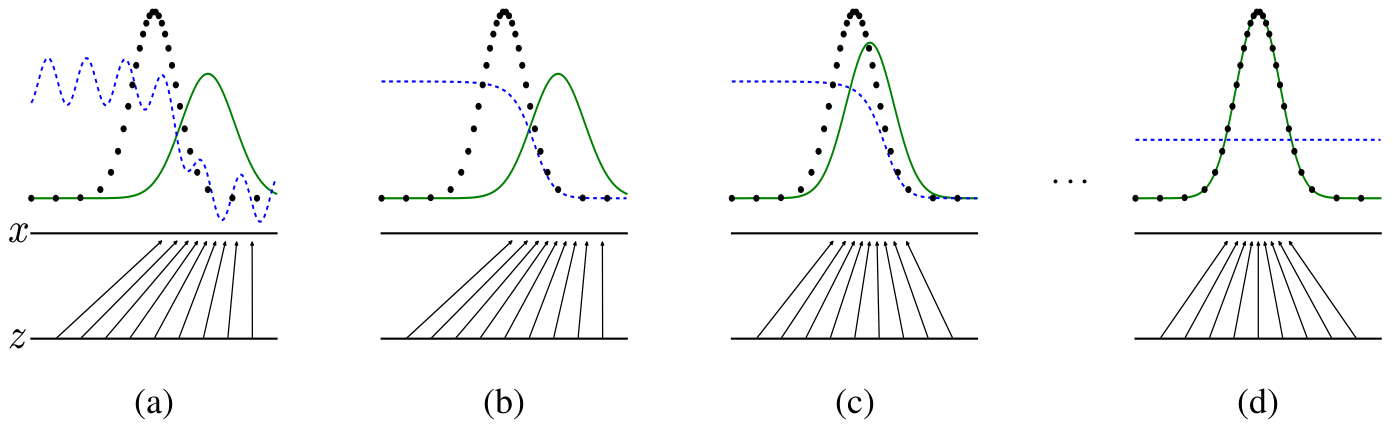
\includegraphics[width=1.0\textwidth]{imgs/Gan training convergence.png}
    \caption{Visualizzazione schematica della convergenza della distribuzione dei dati generati verso quelli reali, e dell'uscita del discriminatore al variare di $\mathbf{x}$.\\
    Si noti che la line nera tratteggiata rappresenta la distribuzione dei dati reali $p_{data}$, mentre la linea verde continua rappresenta la distribuzione dei dati generati $p_{model}$ e
    in fine la linea blu tratteggiata rappresenta l'uscita del discriminatore $D(x)$, al variare di $\mathbf{x}$. 
    I 2 assi in fondo sono rispettivamente, l'asse z i valori casuali di input del generatore con distribuzione fissa, e l'asse x, 
    i valori di input del discriminatore, appartenenti alla distribuzione $\mathbf{p_{data}}$ o $\mathbf{p_{g}}$.\\
    credits: Goodfellow et al. \cite{goodfellow2014generative}}
    \label{fig:gan_training_convergence}
\end{figure}

Nella figura \ref{fig:gan_training_convergence} possiamo vedere diverse fasi dell'addestramento, considerando 4 istanti successivi (a, b, c, d) abbiamo che (a) 
presenta una situazione di apprendimento intermedio in cui il discriminatore comincia ad essere in grado di distinguere con qualche difficoltà i dati reali da quelli
generati e il generatore produce dati piuttosto vicini a quelli reali, in (b) il discriminatore è in grado di distinguere con maggiore precisione i dati reali da quelli
generati, fornendo uno stimolo migliore al generatore, che in (c) è in grado di mappare la distribuzione $\mathbf{p_{z}}$ ad una distribuzione
$\mathbf{p_{g}}$ che tende sempre meglio a quella dei dati reali, infine in (d) possiamo osservare il caso del raggiungimento dell'ottimalità del generatore e dunque la fine dell'addestramento.
In questo caso il discriminatore non è più in grado di distinguere i dati reali da quelli generati, in quanto la distribuzione $\mathbf{p_{g}}$ è sovrapposta 
a quella dei dati reali $\mathbf{p_{data}}$, e si ottiene un'uscita del generatore uguale a 0.5 per ogni valore di input.
La condizione di ottimalità può essere dimostrata, infatti possiamo definire il discriminatore come segue:
\begin{equation}
    \mathbf{D(x) = \frac{p_{data}(x)}{p_{data}(x) + p_{g}(x)}}
\end{equation}

Sapendo che nella condizione ottimale le distribuzioni sono coincidenti $\mathbf{p_{data}(x) = p_{g}(x)}$,
allora considerando $\mathbf{D^*}$ il discriminatore ottimo per un dato $\mathbf{G}$, possiamo scrivere:
\begin{equation}
    \mathbf{D^*(x) = \frac{p_{data}(x)}{p_{data}(x) + p_{g}(x)} = \frac{p_{data}(x)}{2p_{data}(x)} = \frac{1}{2}}
\end{equation}

\subsection{Il gradient vanishing}
Il gradient vanishing è un problema che si verifica nel momento in cui il discriminatore riesce a distinguere con troppa facilità i dati reali da quelli generati,
consideriamo infatti che questa è caratterizzata da un singolo elemento dotato di funzione di trasferimento sigmoide, la quale nel
momento in cui restituisce un valore troppo vicino a 0 o 1, ha il gradiente tendente a zero, e di conseguenza dal momento che l'addestramento 
viene effettuato tramite backpropagation, per quanto visto nel capito precedente anche i gradienti dei layer precedenti tenderanno a zero, e l'addestramento
si arresterà. Vediamo di eseguito la funzione di trasferimento sigmoide e il suo gradiente nel momento in cui tende a saturare:

\begin{figure}[H]
    \centering
    \begin{tabular}{cc}
        % first row
        \subfloat[Saturazione per $\mathbf{y \rightarrow 0}$]{
            \label{fig:sig_grad_0}
            \centering
            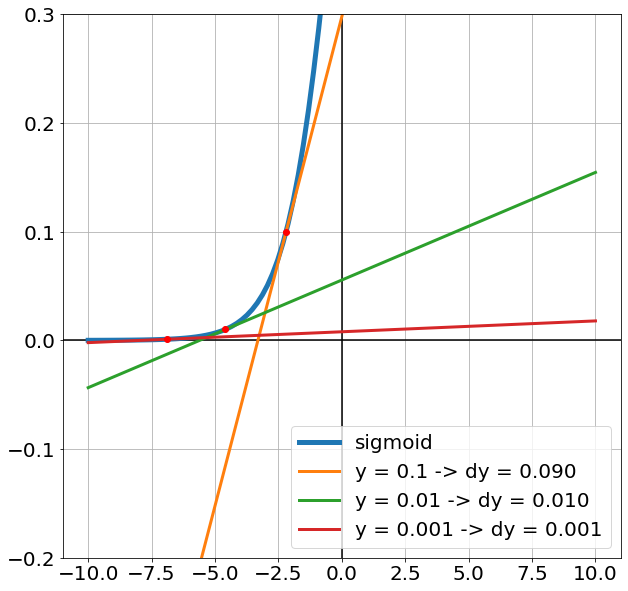
\includegraphics[width=0.4\textwidth]{imgs/graphs/sigmoid_grad_vanish_0.png}
        }  &
        \subfloat[Saturazione per $\mathbf{y \rightarrow 1}$]{
            \label{fig:sig_grad_1}
            \centering
            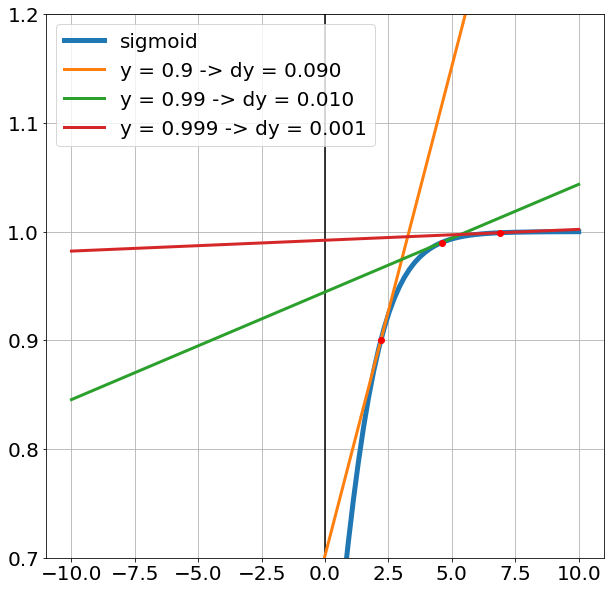
\includegraphics[width=0.4\textwidth]{imgs/graphs/sigmoid_grad_vanish_1.png}
        }  \\
    \end{tabular}
\end{figure}

\subsection{Il mode collapse}
Un'altro problema che affligge i modelli gan è quello del mode collapse, che si verifica quando $\mathbf{G}$ apprende una distribuzione 
che concide con un sottoinsieme di $\mathbf{p_{data}}$. Tale condizione consente comunque di raggiungere
la condizione di ottimalità sopra descritta con $p_{g} \subset p_{data}$, ottenendo comunque $\mathbf{D^*(x) = \frac{1}{2}}$.
Per fare un esempio pratico possiamo considerare ad esempio il dataset Minst che contiene immagini di cifre scritte a mano,
se il generatore impara a generare soltanto cifre dallo 0 al 5 e non quelle dal 6 al 9, siamo in una condizione di mode collapse, 
in quanto parte della distribuzione dei dati non è stata appresa, ma il sistema può comunque raggiungere la condizione di ottimalità.
Nella seguente immagine si ha nella prima riga un esempio di corretto apprendimento mentre nella seconda riga si ha un esempio di mode collapse.
\begin{figure}[H]
    \centering
    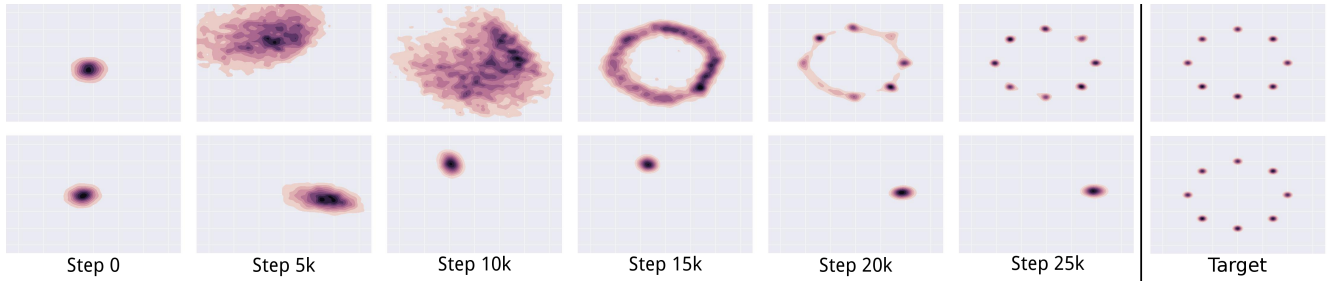
\includegraphics[width=1.0\textwidth]{imgs/mode_collapse.png}
    \caption{Esempio di corretto apprendimento (prima riga) e di mode collapse (seconda riga).\\
    credits: Luke Metz et al. \cite{metz2017unrolled}}
    \label{fig:mode_collapse}
\end{figure}

\subsection{Alcuni risultati}
Vediamo in questa sezione alcuni risultati relativi al modello gan presentato da Goodfellow, relativi a modelli addestrati con
dataset di facce umane in bassa risoluzione e il dataset Minst. In Questi esempi è possibile vedere sulla destra con contorno giallo
alcuni esempi di dati provenienti dal dataset di addestramento, mentre sulla sinistra ci sono gli esempi generati dal modello.

\begin{figure}[H]
    \centering
    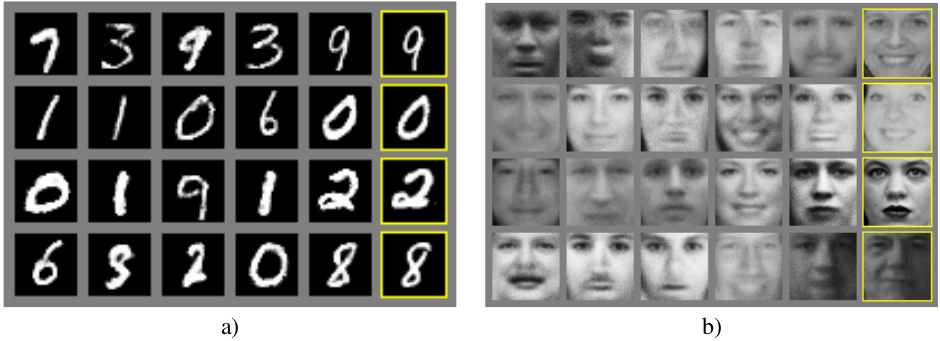
\includegraphics[width=1.0\textwidth]{imgs/first_gan_results.png}
    \caption{Alcuni risultati del modello addestrato in questa ricerca, relativi a un dataset di facce umane in bassa risoluzione (b) e il dataset Minst (a).\\ 
    credits: Goodfellow et al. \cite{goodfellow2014generative}}
    \label{fig:first_gan_results}
\end{figure}

%###############################################################################################################################
%###############################################################################################################################
% DCGAN
\section{DCGAN}
DCGAN è stata la prima pubblicazione, opera di Alec Radford et. al \cite{radford2016unsupervised}, che ha dimostrato l'applicabilità dell'adversarial 
training su modelli convoluzionali, ottenendo buoni risultati, aumentando la dimensione delle immagini rispetto a lavori precedenti e mantenendo una buona
efficienza computazionale. Inoltre in questo articolo sono state mostrate per la prima volta le proprietà aritmetiche vettoriali dello spazio latente 
appreso dal generatore durante l'addestramento.

\subsection{L'architettura del modello}
In realtà questo non è stato il primo tentativo di applicare l'adversarial training su modelli convoluzionali, ma il primo ad avere successo.
Altri ci hanno provato prima ma con scarsi risultati, principalmente a causa dell'instabilità del training, che in questo particolare lavoro è 
stata risolta con l'uso di alcuni interessanti accorgimenti.

Rispetto alle implementazioni classiche di convolutional neural network, una scelta interessante è stata quella di rimuovere completamente 
i layer fully connected, eccetto per l'uscita del discriminatore che è un singolo neurone con funzione di attivazione tanh.
Inoltre sono stati rimossi completamente i layer di pooling, sostituiti da semplici layer di convoluzione con stride 2, in modo da dare al modello
la possibilità di apprendere in autonomia come applicare il downsampling nel discriminatore. Nel generatore invece sono stati usati layer di
convoluzione trasposta con stride 2, per ottenere l'upsampling.
Altre note interessanti riguardano l'uso della funzione di attivazione LeakyReLU per il discriminatore e della ReLU per il generatore, e l'uso
della batch normalization per entrambi i modelli, che ha permesso di ottenere una maggiore stabilità del training.

Di seguito vediamo una delle architetture utilizzate in questo articolo per il generatore:

    \begin{figure}[H]
        \centering
        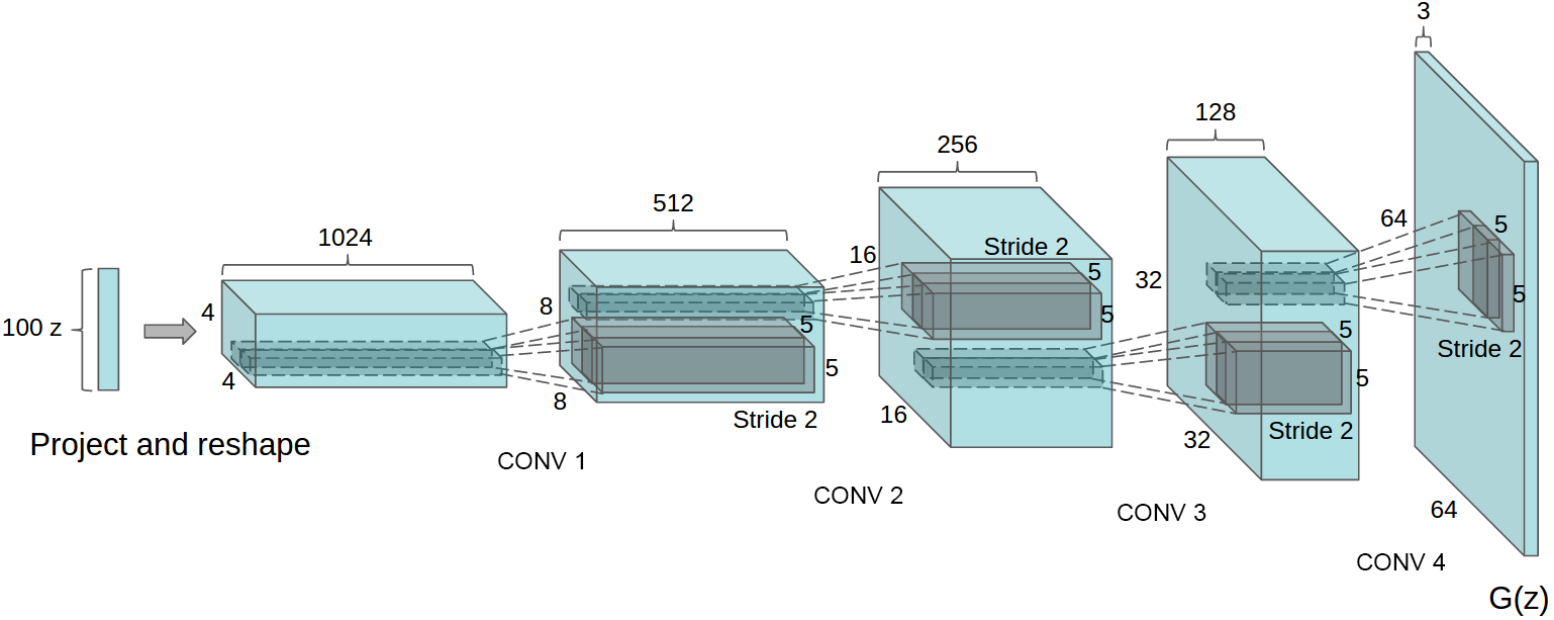
\includegraphics[width=1.0\textwidth]{imgs/DCGAN_generator.png}
        \caption{Architettura del generatore di DCGAN.\\
        credits: Alec Radford et al. \cite{radford2016unsupervised}}
        \label{fig:DCGAN_generator}
    \end{figure}

\subsection{L'algebra vettoriale nello spazio latente Z}
Un'altra proprietà interessante messa in luce da questo articolo sui modelli GAN è il fatto che durante l'addestramento, benche l'input 
$\mathbf{z} \sim \mathbf{p_{z}}$ sia un vettore casuale proveniente da una distribuzione tipicamente gaussiana, il generatore
mostra delle proprietà di auto organizzazione, associando arbitrariamente diverse zone dello spazio latente a diverse caratteristiche 
appartenenti alla distribuzione dei dati reali.
Questo spazio autorganizzato mostra addirittura delle proprietà aritmetiche vettoriali, in quanto sembra possibile effettuare 
operazioni di somma e sottrazione tra i vettori in Z, ed ottenere dei risultati coerenti in termini di immagini. Le stesse semplici operazioni 
effettuate a livello di immagine non danno risultati paragonabili, per tale ragione questo comportamento è indice del fatto che il modello
apprende una rappresentazione dei dati nello spazio latente in maniera profonda e relativa alle caratteristiche che essi presentano, in 
maniera del tutto non supervisionata.

Vediamo un esempio tratto dallo stesso articolo, creato attraverso un modello addestrato su un dataset di facce umane.
Nell'esempio vengono presi 3 vettori per 3 distinte aree di Z: "donna sorridente", "donna seria", "uomo serio" e viene fatta la media 
di questi vettori, ottenendo ancora un vettore che possiede le stesse caratteristiche, ciò indica che queste tre aree sembrano avere una sorta di 
convessità, i vettori mediati vengono poi utilizzati per estrarre la caratteristica "sorridente" e aggiungerla al vettore appartenente all'area "uomo serio",
ottenendo un nuovo vettore che rappresenta un uomo sorridente.
Ciò significa che nello spazio Z è possibile isolare delle caratteristiche e combinarle tra loro per ottenere nuove immagini, lo svantaggio purtroppo
è che lo spazio Z è caratterizzato da una dimensionalità molto elevata, e inoltre queste zone associate a caratteristiche specifiche presentano una elevata
non linearità, per cui in generale è difficile effettuare operazioni di questo tipo con un buon controllo del risultato.

    \begin{figure}[H]
        \centering
        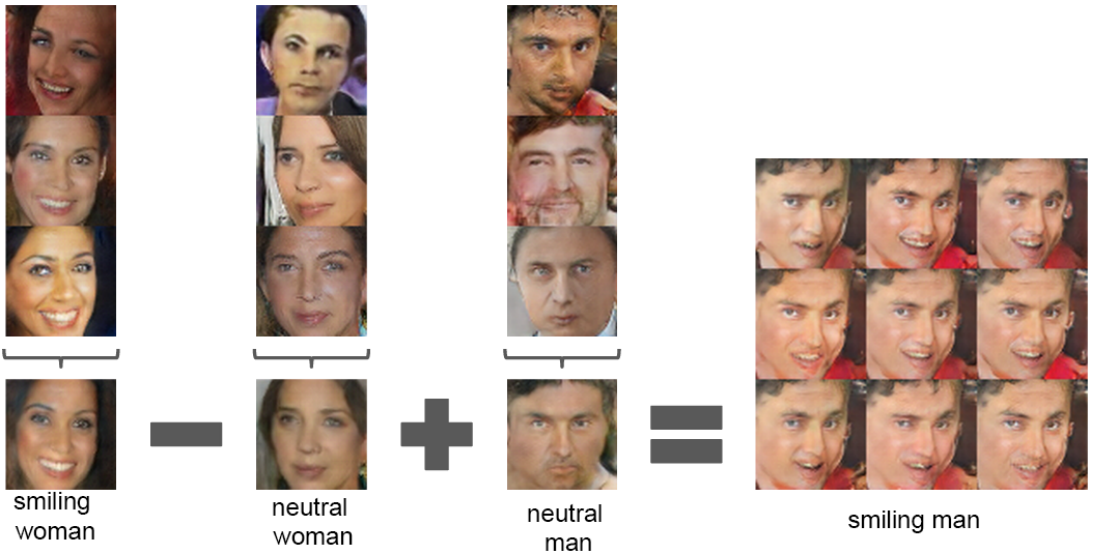
\includegraphics[width=1.0\textwidth]{imgs/DCGAN_vectorial_algebra.png}
        \caption{Esempio di algebra vettoriale nello spazio latente Z.\\
        credits: Alec Radford et al. \cite{radford2016unsupervised}}
        \label{fig:DCGAN_vectorial_algebra}
    \end{figure}
\section{Wasserstein GAN}
TODO
\section{Stylegan}
TODO



